\chapter{DAGs}
\label{chapt:DAGs}

Introduciamo come primo argomento i DAGs o Directed Acyclic Graph, questi servono per schematizzare relazioni di causalità, che non verrà  
definità rigorosamente ora ma affrontata nel capitolo \ref{chapt:PotentialOM}.
Un DAG è un grafo formato da vertici che rappresentano le variabili in analisi e da archi che rappresentano la relazione di causalità le variabili. Viene detto aciclico perché partendo da un vertice e seguendo gli archi non si può tornare su  quel vertice. Questi grafi non sono in grado di descrivere causalità reciproca simultanea $A \leftrightarrow B $  o feedback loop $A \rightarrow B \rightarrow A$ a meno che si inserisca un ulteriore vertice con lo stesso nome, anche se in questi casi non si consiglia di utilizzare questo tipo di grafici
\citep{cunningham2021causal}.

\begin{figure}[ht]
  \subcaptionbox{Non valid DAG}[.22\linewidth]{%
	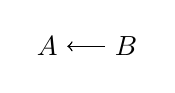
\begin{tikzpicture}
		\node (A) at (0,0) {$A$};
    		\node (B) at (1,0) {$B$};
    		\path[<-] (A) edge (B);
    		\path[->] (B) edge (A);
	\end{tikzpicture}
  }%
  \subcaptionbox{Non valid DAG}[.22\linewidth]{%
	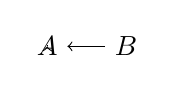
\begin{tikzpicture}
		\node (A) at (0,0) {$A$};
    		\node (B) at (1,0) {$B$};
    		\path[<-] (A) edge (A);
    		\path[->] (B) edge (A);
	\end{tikzpicture}
  }
  \subcaptionbox{Valid DAG}[.22\linewidth]{%
	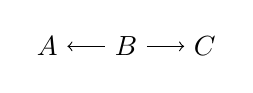
\begin{tikzpicture}
		\node (A) at (0,0) {$A$};
    		\node (B) at (1,0) {$B$};
    		\node (C) at (2,0) {$C$};
    		\path[<-] (A) edge (B);
    		\path[->] (B) edge (C);
    		
	\end{tikzpicture}
  }%
	\label{validDAG}

\end{figure}
(I grafi sono da rifare)

Bisogna inoltre dire che i DAGs, essendo dei grafi sono di natura più sintetici, contengono molte informazioni non solo grazie agli archi disegnati ma anche grazie a quelli \textbf{non} disegnati, ad esempio il DAG \ref{validDAG} implica che $A \perp\!\!\!\perp C$ visto che non esiste un arco che li colleghi. 

 %Bisogna essere molto vigili delle assunzione nascoste di un DAG.



\section{Vertici e Archi}
Fare breve cappello

\subsection{Vertici}

Poniamo la C come la variabile \textit{outcome} cioè la variabile di interesse per l'indagine (la salute dopo un determinato intervento). Poniamo A come la variabile \textit{exposure} cioè quella di cui vogliamo quantificare l'effetto causale sulla variabile \textit{outcome} (per esempio che tipo di intervento viene proposto). Analizziamo quindi un singolo vertice in questo caso B, gli unici modi in cui si può collegare ad A e C sono i seguenti: 
\begin{figure}[H]
\centering    
	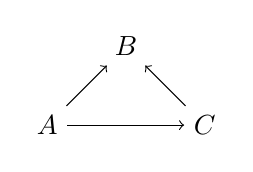
\begin{tikzpicture}
		\node (A) at (0,0) {$A$};
    		\node (B) at (1,1) {$B$};
    		\node (C) at (2,0) {$C$};
		\path[->] (A) edge (B);
    		\path[<-] (B) edge (C);
    		\path[->] (A) edge (C);
	\end{tikzpicture}
\caption{DAG: Common effect}
\label{DAG:Common effect}
\end{figure} 
\begin{figure}[H]
	\centering
	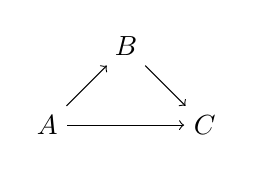
\begin{tikzpicture}
		\node (A) at (0,0) {$A$};
    		\node (B) at (1,1) {$B$};
    		\node (C) at (2,0) {$C$};
    		\path[->] (A) edge (B);
    		\path[->] (B) edge (C);
		\path[->] (A) edge (C);
	\end{tikzpicture}
\caption{DAG: Mediator}
\label{DAG:Mediator}
\end{figure} 
\begin{figure}[H]
	\centering
	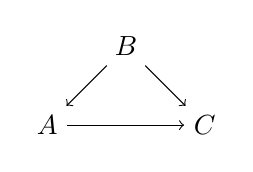
\begin{tikzpicture}
		\node (A) at (0,0) {$A$};
    		\node (B) at (1,1) {$B$};
    		\node (C) at (2,0) {$C$};
    		\path[<-] (A) edge (B);
    		\path[->] (B) edge (C);
    		\path[->] (A) edge (C);
	\end{tikzpicture}
\caption{DAG: Common cause}
\label{DAG:Common cause}
\end{figure}
Dunque B nel grafico \ref{DAG:Common effect} viene chiamato \textit{collider}, mentre nei grafici \ref{DAG:Mediator} e \ref{DAG:Common cause} viene definito \textit{non collider}, mentre solo \ref{DAG:Common cause} come \textit{confounder}.
Infatti se volessimo quantificare la relazione causale tra A e C quando B è un \textit{non collider} o  un \textit{confounder} risulta più difficoltoso perchè sappiamo che B introduce  sistematicamente correlazioni spurie tra A e C (bisogna capire meglio come affrontare i mediators [bisogna controllarli?], osservazione più giusta per i ). Invece nel caso mostrato in figura \ref{DAG:Common effect} potremmo interpretare il $\hat{\delta}$ della regressione lineare:
\begin{equation}
C_i= A_i\delta + \epsilon_i
\end{equation}
come quantificazione dell'effetto causale che A ha su C, questo lo possiamo affermare solo dopo aver confermato che effettivamente:
\begin{itemize}
\item il grafo soddisfa \textit{Backdoor criterion} ( paragrafo \ref{sect:backdoor})
\item La direzione della causalità è corretta
\end{itemize}

\subsection{Archi}
definizione di path
definizione di open backdoor 
elenco di tutte le path possibili  con esempio




% magari metterli di fianco
%\begin{figure}[ht]
%  \subcaptionbox{First subfigure}[.22\linewidth]{%
%	\begin{tikzpicture}
%		\node (A) at (0,0) {$A$};
%    		\node (B) at (1,0) {$B$};
%    		\node (C) at (2,0) {$C$};
%    		\path[<-] (A) edge (B);
%    		\path[->] (B) edge (C);
%	\end{tikzpicture}
%  }%
%  \hfill
%  \subcaptionbox{Second subfigure}[.22\linewidth]{%
%	\begin{tikzpicture}
%		\node (A) at (0,0) {$A$};
%    		\node (B) at (1,0) {$B$};
%    		\node (C) at (2,0) {$C$};
%    		\path[<-] (A) edge (B);
%    		\path[->] (B) edge (C);
%	\end{tikzpicture}
%  }
%  \subcaptionbox{First subfigure}[.22\linewidth]{%
%	\begin{tikzpicture}
%		\node (A) at (0,0) {$A$};
%    		\node (B) at (1,0) {$B$};
%    		\node (C) at (2,0) {$C$};
%    		\path[<-] (A) edge (B);
%    		\path[->] (B) edge (C);
%	\end{tikzpicture}
%  }%
%
%\end{figure}

\section{Back door criterion}
\label{sect:backdoor}


\section{Collider Bias}
\begin{figure}[H]
\centering
	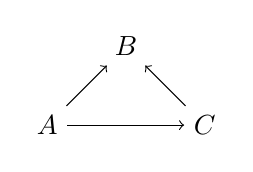
\begin{tikzpicture}
		\node (A) at (0,0) {$A$};
    		\node (B) at (1,1) {$B$};
    		\node (C) at (2,0) {$C$};
		\path[->] (A) edge (B);
    		\path[<-] (B) edge (C);
    		\path[->] (A) edge (C);
	\end{tikzpicture}
\caption{DAG:collider bias}
\label{DAG:Colliderbias}
\end{figure} 

